\documentclass[11pt]{article}
\usepackage[a4paper, hmargin={2.8cm, 2.8cm}, vmargin={2.5cm, 2.5cm}]{geometry}
\usepackage{eso-pic} % \AddToShipoutPicture
\usepackage{graphicx} % \includegraphics
\usepackage{tabto}
\usepackage{enumerate}
\usepackage{txfonts}
\usepackage{graphicx}
\usepackage{float}
\usepackage{amsmath}

%% Change `ku-farve` to `nat-farve` to use SCIENCE's old colors or
%% `natbio-farve` to use SCIENCE's new colors and logo.
\def \ColourPDF {include/ku-farve}

%% Change `ku-en` to `nat-en` to use the `Faculty of Science` header
\def \TitlePDF   {include/ku-en}  % University of Copenhagen

\title{
  \vspace{3cm}
  \Huge{Some Title} \\
  \Large{More elaborate subtitle}
}

\author{
  \Large{Bjarke Kingo Iversen}
  \\ \texttt{bjarkekingo50@gmail.com} \\\\
  \Large{Susanne Truong}
  \\ \texttt{suzze-t@hotmail.com}
}

\date{
    \today
}

\begin{document}

\AddToShipoutPicture*{\put(0,0){\includegraphics*[viewport=0 0 700 600]{\ColourPDF}}}
\AddToShipoutPicture*{\put(0,602){\includegraphics*[viewport=0 600 700 1600]{\ColourPDF}}}

\AddToShipoutPicture*{\put(0,0){\includegraphics*{\TitlePDF}}}

\clearpage\maketitle
\thispagestyle{empty}

\newpage

%% Write your dissertation here.
\section{Abstract}
\newpage
\tableofcontents
\newpage
%%%%%%%%%%%%%%%%%%%%%%%%%%%%% Introduction %%%%%%%%%%%%%%%%%%%%%%%%%%%%%
\section{Introduction}
It is widely known that it can be time-consuming to choose the wrong path, if you want to travel from one city to another. It will most certainly be faster to aboard the train from Chicago to Seattle, rather than going through Los Angeles before heading to Seattle. Choosing the right path will therefore save a lot of time.\\
The problem herein is that its in lots of cases is nowhere intuitive which path that guarantees the consumation of time to be minimal. We probably can't withstand the big amounts of information if we should compute the shortest path, through millions of combinations by ourselves. For computersystems to choose such a path, they'd need a method for calculating such, an algorithm.\\
Different shortest-path algorithms are known to solve such problems theoretically. We'll examine the theory behind these, and analyse the complexity to see whether the time-complexity given by Bellmann-Ford and Dijkstras algorithms holds in real life implementations, by implementing them with both a binary and a fibonacci-heap in C++, thus finally to match them all up against each other.\\
We'll as well analyse and implement the A*-algorithm to see how well dijkstra match up against this on euclidean planar graphs. Since we're primarily interested in road-maps, we won't consider negative weights.\\

\section{Problem definition}
To examine and benchmark the complexity of different shortest-path algorithms, e.g. Dijkstra, Bellmann-Ford, and A* Search. We will do this by implementing and comparing them using different data structures and libraries. Finally we will compare the results of these experiments with the theoretical bounds.

%%%%%%%%%%%%%%%%%%%%%%%%%%%%%%% Notation %%%%%%%%%%%%%%%%%%%%%%%%%%%%%%%
\section{Notation}
A short list of notations used throughout the thesis:
\begin{itemize}
\item $G(V,E)$ = Graph, consisting of set of vertices V, and set of edges E
\item $s$ = Designated to be the source vertex s
\item $w(u,v)$ = Weighted distance from vertix u to v
\item $d[v]$ = The weigth of the current shortest path from s to v. $d[v]$ is initlized to be $\infty$ for all vertices besides the source vertex. $d[s]$ is initialized to be 0.
\item $\pi[v]$ = Predecessor/parent vertex to v in the current shortest path. $\pi[v]$ is initialized to be NIL. This is set to a vertex once/if a path is discovered from s to v.
\item $\delta(u,v)$ = the weigth of the shortest path from u to v.
\item lg(n) = $log_{2}$(n).
\item $v_{1}, v_{2}, ..., v_{k}$ a path from some start-vertice containing k vertices in successing order. 
\end{itemize}

%%%%%%%%%%%%%%%%%%%%%%%%%%% Shortest Paths %%%%%%%%%%%%%%%%%%%%%%%%%%%
\section{On Shortest Paths}
In the shortest path problem, a graph $G = (V,E)$ is given, where $V$	
is the set of vertices, and $E$ is the set of edges. Each edge
connects two vertices and contains a weight, indicating the cost of
moving between these vertices. By using a shortest path algorithm, we
can find a shortest path $P = {v_{1}, v_{2}, ..., v_{k}} \in V$ from a
given source vertex $s \in V$ to all other vertices $v \in V$. I.e.,
we want to find a path, where the total weight of the visited edges is
minimal.\\
We can compute the total sum of weights in a path P containing k vertices thus:\\
$$w(P) = \displaystyle\sum_{i=1}^{k} w(v_{i-1},v_i)$$

%%%%%%%%%%%%%%%%%%%%%%%%%%%%% Relaxation %%%%%%%%%%%%%%%%%%%%%%%%%%%%%
\noindent
\subsection{Initialization \& Relaxation}
When searching for the shortest path from a source vertex $s$ to a
vertex $v$, a shortest-path estimate $d[v]$ is preserved for each
vertex $v \in V$. To initialize the estimate and predecessor for all vertices, the following function is used:\\

\textbf{INITIALIZE-SINGLE-SOURCE$(G, s)$}
\begin{enumerate}
\NumTabs{24}
\setlength\itemsep{0em}
\item \textbf{for } each vertex $v \in G.V$
\item \tab{$d[v] = \infty$}
\item \tab{$\pi[v] = NIL$}
\item $d[s] = 0$
\end{enumerate}
The shortest-path estimate for the source is 0, since this is where the algorithm begins. The other vertices' distance is set to $\infty$, since the path from $s$ to a vertex $v$ is unknown at start. Not knowing the path also results in the predecessor being unknown, which is why $\pi[v]$ is set to NIL.\\
At first, $d[v]$ will be an overestimate, but if we see that the shortest path to $v$ can be improved by going through a vertex $u$, we update the estimate $d[v]$ with the new and lower cost. As better paths are found, we will eventually get the correct estimate and find the shortest path, if it exists. This technique is called relaxation and is used by the three algorithms that we will talk about later. The pseudocode for relaxing an edge $(u,v) $ is shown below:\footnote{Introduction to Algorithms, pg. 649}\\

\textbf{RELAX$(u, v, w)$}
\begin{enumerate}
\NumTabs{24}
\setlength\itemsep{0em}
\item \textbf{if } $d[v] > d[u] + w(u,v)$
\item \tab{$d[v] = d[u] + w(u,v)$}
\item \tab{$\pi[v] = u$}
\end{enumerate}
If the current distance from a source to the vertex $v$ is larger than the path going through vertex $u$ to $v$, the estimate is updated. And the predecessor for $v$ will then be $u$. The figure below illustrates the procedure of relaxing an edge $(u,v)$. Before relaxing the edge, we have that $d[v] > d[u] + w(u,v)$. $d[v]$ therefore gets decreased. Had the condition not been true, $d[v]$ would have remained at the same value of 10. 

\begin{figure}[H]
\centering
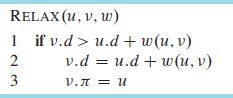
\includegraphics[scale=0.4]{relaxation.png}
\caption{Relaxing an edge $(u,v)$}
\end{figure}


%%%%%%%%%%%%%%%%%%%%%%%%%%%%% Properties %%%%%%%%%%%%%%%%%%%%%%%%%%%%%
\section{Properties of shortest path algorithms}
The shortest path algorithms that we have talked about will always find a shortest path, if it exists. This can be proved by looking at the properties that shortest paths and relaxation have:\footnote{Introduction to Algorithms, pg. 650}

\subsection{Triangle inequality}\\
The triangle inequality lemma is a geometric property of triangles which states that the sum of two lengths of any two sides must be greater than or equal to the remaining side. That is, for any triangle with sides $\{x,y,z\}$, we have that $z \leq x+y$.\\\\
Applied to the shortest path problem we have that for any edge $(u,v) \in E$, we have $\delta(s,v)\leq \delta(s,u) + w(u,v)$ (\textbf{Lemma 1}). Thus the shortest path from s to v must be less than or equal to the shortest path from s to u added to the weigth from u to v.\\
\subsection{Upper-bound property}\\
The upper-bound property says that our estimate for the shortest distance to v is always greater than or equal to the actual shortest path from s to v, for all vertices v$\in$ V.\\\\
That is $\forall v \in V.(d[v]\geq \delta(s,v))$. Once our estimate holds the actual value for the shortest path, the estimate never changes (\textbf{Lemma 2}).\\
\subsection{No-path property} (\textbf{Corollary to Lemma 2})\\
If there is no path from s to v, then we always have $d[v] = \delta(s,v) = \infty$.\\
\subsection{Convergence property}\\
The convergence property ensures us that if we from s, at sometime has u to v is the shortest path in G for some u,v $\in$ V, and if the estimated shortest path to u actually is the shortest path, we'd then have (prior to relaxing the edge (u,v)) that the estimated shortest path to v must be the shortest path to v at all times afterward.\\\\
That is, if $s\rightsquigarrow u\rightarrow v$ is a shortest path, and if $d[u] = \delta(s,u)$, then $d[v] = \delta(s,v)$ is assured at all time afterward (\textbf{Lemma 3}).\\
\subsection{Path-relaxation property}\\
Our path-relaxation property ensures that the relaxation of a shortest path p will derive that the distance to the k'th vertix in p is equal to the shortest path to vertix k.\\\\
Let $p = \{v_{1}, v_{2},\cdots ,v_{k}\}$ be a shortest path that goes from $v_{1}$ to $v_{k}$. If the edges are relaxed in the order $(v_{1},v_{2}), (v_{2},v_{3}), \cdots , (v_{k-1}, v_{k})$, then $d[v_{k}] = \delta(s,v_{k})$ once the whole path is relaxed \footnote{Shortest Paths: 6.006 Intro to Algorithms, March 30 2011, Recitation 14. MIT}(\textbf{Lemma 4}).\\
\subsection{Predecessor-subgraph property}\\
The predecessor-subgraph/parent-subgraph property ensures that once the shortest path to v is computed for all vertices v, the predecessor subgraph is a shorted-paths tree rooted at s.\\\\
Such that once $\forall v \in V.(d[v] = \delta(s,v))$ the predecessor subgraph that contains all the vertices with a finite distance from s, but with only edges that connects v to $\pi[v]$ is a shortest-path tree\footnote{Shortest Paths: 6.006 Intro to Algorithms, March 30 2011, Recitation 14. MIT} (\textbf{Lemma 5}).
\end{itemize}

\includegraphics[scale=0.5]{grimtSP.png}


%%%%%%%%%%%%%%%%%%%%%%%%%%%% Dijkstra proof %%%%%%%%%%%%%%%%%%%%%%%%%%%%
\newpage
\section{Correctness of Dijkstra's algorithm}\\
To prove that Dijkstra's algorithm work, we will perform an induction proof. Let $S$ be the set of vertices, whose shortest path have been found, $S=V-Q$.\\\\
\textbf{Loop Invariant}\\
$\forall v\in S.(d[v] = \delta(s,v))$\\\\
\textbf{Initialization}\\
Let \textbf{Size}(S)=1. This is true when S only holds the source vertex, $S = \{s\}$. Since $d[s]=0=\delta(s)$, the invariant holds.\\\\
\textbf{Maintenance}\\
Let $v$ be the latest vertex added to $S$. Let $S'$ = $S \cup \{v\}$. For each vertex in $S'$, we want to have that our loop invariant holds. EXTRACT-MIN(Q) ensures that the correct distance label gets extracted from $Q$ and put into $S$. We therefore only need to show that $d[v]=\delta(s,v)$ for $S'=S \cup \{v\}$. To prove this, we will perform a contradiction. Assume that there exists a shortest path $P^{sv}=(v_s, v_2, ..., v_v)$ from the source vertex $s$ to target vertex $v$ that has length $$w(P^{sv}) < d[v]$$
Before adding $v$ to $S$, the path $P^{sv}$ connects a vertex $u\in S$ to the vertex $v\in V-S$ through one or more edges. Let $y$ be the first vertex along $P^{sv}$ that is an element of $V-S$. Let $x\in S$ be $y's$ predecessor along the path $P^{sv}$. Let $P^{sx}=(v_s, v_2, ..., v_x)$ be a subpath of $P^{sv}$ from vertex $s$ to $x$. Once we want to add $v$ to $S$, we have already gone through the edge $(x,y)$: $$w(P^{sx}) + w(x,y) \leq w(P^{sy})$$
Due to vertex $y$ being successor to vertex $x$, Dijkstra's algorithm must have relaxed $(x,y)$, so $$d[y]\leq d[x]+w(x,y)$$\\
Now we have that $d[y] = \delta(s,y)$. But when EXTRACT-MIN(Q) is called in the pseudocode (line 5), it returns vertex $v$ instead of $y$, even though both are in the set $V-S$. This means $v$ must have the shortest distance label, so $$d[v] \leq d[y]$$
This means that $$d[v] = d[y]$$ This contradicts our original assumption of $w(P^{sv}) < d[v]$, since we already have the shortest path $$d[v] = w(P^{sy}) \leq w(P^{sv})$$.
$$(w(P^{sv}) \geq d[v]) \neq (w(P^{sv}) < d[v])$$\\
\textbf{Termination}\\
We terminate once $Q = V-S =\O$. If $\exists t \in S$, we can backtrace the predecessors to obtain $\delta(s,t)$. Otherwise, we have that $\delta(s,t) = \infty$ by the no-path property.\\


%%%%%%%%%%%%%%%%%%%%%%%%%%%%% Bellman-Ford %%%%%%%%%%%%%%%%%%%%%%%%%%%%%
\section{Bellman-Ford algorithm}
Bellman-Ford algorithm solves the single-source shortest-path problem in the case where edge weights may be negative.\\
If there is a negative cycle, the cost of the shortest path is decreased every time the algorithm runs through the negative cycle. By doing this numerous times, we can receive arbitrarily negative weights, thus making the cost undefined.\\
If no such cycle is found, the algorithm succesfully computes the shortest paths from s to each vertex v $\in$ V by iteratively decreasing d[v] by relaxing edges $\in$ E until $\delta(s,v)$ is found.\\
The algorithm returns true if and only if the graph has no negative-weight cycles reachable from the source vertex.\\
Otherwise it terminates and returns false upon finding such a cycle.\\\\
The pseudocode for Bellman-Ford's algorithm can be seen below:\footnote{Introduction to Algorithms, pg. 651}\\

\textbf{BELLMAN-FORD$(G, w, s)$}
\begin{enumerate}
\NumTabs{24}
\setlength\itemsep{0em}
\item \textbf{INITIALIZE-SINGLE-SOURCE}$(G, s)$
\item $\textbf{for } i = 1 \textbf{to } |V[G]| -1$
\item \tab{$\textbf{for }$ each edge $(u,v) \in E[G]$}
\item \tab{}\tab{\textbf{RELAX}(u, v, w)}
\item $\textbf{for }$ each edge $(u,v) \in E[G]$
\item \tab{$\textbf{if } d[v] > d[u] + w(u,v)$}
\item \tab{}\teb{\textbf{RETURN } FALSE}
\item \textbf{RETURN } TRUE
\end{enumerate}




%%%%%%%%%%%%%%%%%%%%%%%%%%%%%%%% Heaps %%%%%%%%%%%%%%%%%%%%%%%%%%%%%%%%%
\section{Heaps}
In the following section, we will describe the priority queues we use for our interpretation of the Dijkstra's and A* search algorithm.\\
\subsection{Binary Min-Heaps}
A binary heap is a tree-like data-structure, where each node contains 2 child nodes, in a balanced way, such that the last parent node may have 1 or 2 child nodes. The height of a tree containing n nodes is $\lfloor lg(n) \rfloor$. When the height of the tree grows linearly the amount of nodes therefor grow exponentially. The amount of nodes in af tree of height n would therefor be between $2^n$ and $2^{n+1}-1$. But lets use the approximation of $2^n$ for now.\\\\
\textbf{BILLEDE AF HOB + ARRAY HER}\\
By using the properties of the binary heap, we can compute some nodes, given an index thus:\\
\begin{center}
$\pmb{Parent(i) = \lfloor i/2 \rfloor}$\\
\pmb{$Left(i) = 2i$}\\
\pmb{$Right(i) = 2i+1$}\\
\end{center}
In the binary min-heap we have that the value of the nodes are in decreasing order when moving from a leaf node, up through the parent-nodes. Symmetrically, we have that the values are in ascending order when moving down arbitrarily through the nodes. That is, we have for all nodes that \pmb{Min-heap[Parent(i)] $\leq$ Min-heap[i]}.\\\\
For our shortest-path algorithms to work on the binary-heap datastructure, we need 3 functions:
\subsubsection{Decrease-Key}
By calling our \textbf{Relaxation} we use the Decrease-Key method, which is the method of decreasing the value of a given node i, if our relaxation can improve the distance-estimate. It changes the value of node i to our key and as long as the Parent(i) is larger than i, it swaps i with Parent(i), and assigns the the index i to the index Parent(i).\\\\
\textbf{DECREASE-KEY(Min-Heap, i, key)}
\begin{enumerate}
\NumTabs{24}
\setlength\itemsep{0em}
\item Min-Heap[i] = key
\item \textbf{while } i $>$ 1 and Min-Heap[Parent(i)] $>$ Min-Heap[i]
\item \tab{\textbf{Swap}(Min-Heap[i], Min-Heap[Parent(i)])}
\item \tab{i = Parent(i)}
\end{enumerate}
\subsubsection{Insert}
Insertion is the method of inserting a new node into our min-heap.\\
When we insert, we add 1 extra space to our heap, and inserts it here.\\
We run our Decrease-Key again to have our new node have the right place in the Min-Heap.\\\\
\textbf{INSERT(Min-Heap, key)}
\begin{enumerate}
\NumTabs{24}
\setlength\itemsep{0em}
\item \textbf{Size}(Min-Heap) = \textbf{Size}(Min-Heap) + 1
\item Min-Heap[\textbf{Size}(Min-Heap)] = NIL
\item DECREASE-KEY(Min-Heap, \textbf{Size}(Min-Heap), key)
\end{enumerate}
We can in the ordinary Dijkstras algorithm do this in a more clever way which will be discussed in the '\textbf{Running time analysis}'-section
\subsubsection{Extract-Min}\\
By calling our \textbf{Extract-Min} we take out the Min-Heap[1], which is the root of our Min-Heap and will be guaranteed by Insert and Decrease-Key to have the minimum-value. When we do this, we put up our terminal node in the root, decreases the heap-size by 1 and balances it by swapping it with the smallest child-node recursively until we have it in the right spot.\\\\
\textbf{BALANCE-MIN-HEAP(Min-Heap, i)}
\begin{enumerate}
\NumTabs{24}
\setlength\itemsep{0em}
\item L = \textbf{Left}(i)
\item R = \textbf{Right}(i)
\item \textbf{if } L $\leq$ \textbf{Size}(Min-Heap) \textbf{and} (Min-Heap[L] $<$ Min-Heap[i])
\item \tab \textbf{then } smallest = L
\item \tab \textbf{else } smallest = i
\item \textbf{if } R $\leq$ \textbf{Size}(Min-Heap) \textbf{and} (Min-Heap[R] $<$ Min-Heap[smallest])
\item \tab \textbf{then } minimum = R
\item \textbf{if } minimum $\neq$ i
\item \tab \textbf{then } \textbf{Swap}(Min-Heap[i], Min-Heap[minimum])
\item \tab \tab \textbf{BALANCE-MIN-HEAP}(Min-Heap, minimum)
\end{enumerate}
\  \\
\textbf{EXTRACT-MIN(Min-Heap)}
\begin{enumerate}
\NumTabs{24}
\setlength\itemsep{0em}
\item \textbf{if } \textbf{Size}(Min-Heap) $<$ 1
\item \tab raise error "Heap underflow"
\item min = Min-Heap[1]
\item Min-Heap[1] = Min-Heap[\textbf{Size}(Min-Heap)]
\item \textbf{Size}(Min-Heap) = \textbf{Size}(Min-Heap) - 1
\item \textbf{BALANCE-MIN-HEAP}(Min-Heap, 1)
\item \textbf{return} min
\end{enumerate}
\  \\
\subsection{Fibonacci-Heaps}
\newpage
%%%%%%%%%%%%%%%%%%%%%%%%%%%%%%% Dijkstra %%%%%%%%%%%%%%%%%%%%%%%%%%%%%%%
\section{Dijkstra's algorithm}
Dijkstra's algorithm takes a weighted graph $G = (V, E)$ and finds the shortest path from a single source to each other vertex in the graph. To keep track of the vertices, the algorithm maintains two sets of vertices. The set $S$ consists of vertices, where the optimal shortest-path estimate from the source $s$ has been figured. The other set $Q$ is a minimum priority queue that contains the remaining vertices, i.e. $Q = V - S$. The algorithm will repeatedly extract a vertex with the minimum shortest-path estimate from $Q$ and add it to $S$, until all vertices have been discovered.\\

\noindent 
\textbf{Assumptions}\\
For Dijkstra's algorithm to work, we must assume that the graph contains no negative weights. Once a vertex has been extracted from the min-priority queue, Dijkstra's algorithm will assume that the shortest path to that vertex has been found. This means the algorithm will never have to relax this vertex again. However, if there is a negative-weighted edge somewhere, the algorithm may find a wrong shortest-path.\footnote{http://stackoverflow.com/questions/13159337/why-doesnt-dijkstras-algorithm-work-for-negative-weight-edges} An example can be seen in the following figure:\\

\begin{figure}[H]
\centering
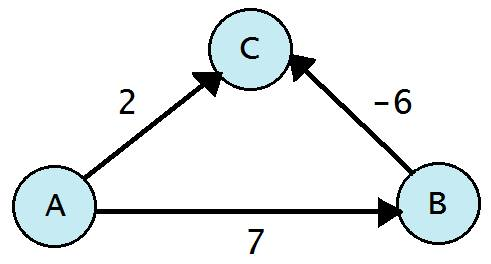
\includegraphics[scale=0.3]{neg-weight.png}
\caption{A graph with negative weights}
\end{figure}

\noindent In this figure, the graph consists of three vertices $A, B,$ and $C$. Dijkstra's algorithm starts at the source $A$ and will first extract $C$, since it has the shortest-path estimate of 2. Afterwards, the algorithm extracts the last vertex $B$ and terminates. Had it however tried to relax the negative edge between $B$ and $C$, a shorter path of $7 - 6 = 1$ would have been discovered. The result is therefore incorrect due to dijkstra utilizing the greedy property of \textbf{Lemma 1}, thus that $\forall (u,v) \in E.(w(u,v) \geq 0)$. \\

\noindent
(\textbf{Does the graph have to be connected???}\\
A connected graph means that for all $v \in V $,a vertex $v$ will be reachable from another vertex $w$ through an edge. If the graph is disconnected, some vertices will be unreachable, thus making some shortest paths infinite, if we try to reach these vertices.)\\\\


\noindent
\textbf{How Dijkstra's algorithm works}:\\
The pseudocode for Dijkstra's algorithm can be seen below:\footnote{Introduction to Algorithms, pg. 658}\\

\textbf{DIJKSTRA$(G, w, s)$}
\begin{enumerate}
\NumTabs{24}
\setlength\itemsep{0em}
\item INITIALIZE-SINGLE-SOURCE$(G, s)$
\item $S = $ \O
\item $Q = G.V$
\item $\textbf{while } Q \neq$ \O
\item \tab{$u = $ EXTRACT-MIN$(Q)$}
\item \tab{$S = S \cup \{u\}$}
\item \tab{\textbf{for} each vertex $v \in G.Adj[u]$}
\item \tab{}\tab{RELAX$(u,v,w)$}
\end{enumerate}

\noindent The graph is initialized in line 1 by calling INITIALIZE-SINGLE-SOURCE. For each vertex $v \in G.V$, the function sets the shortest-path estimate to $\infty$ and predecessor to NIL. $d[s]$ is set to 0. Dijkstra's algorithm maintains two sets, $S$ and $Q$. The set $S$ contains the vertices, whose final shortest-path estimates have been determined. In the beginning, no paths have been determined and thus $S$ will be empty (line 2). The min-priority queue $Q$ contains the vertices, whose shortest paths have not been found yet and is keyed by the vertices' current shortest-path estimates. In other words, the set of vertices in the graph is equal to the two sets, $V = S + Q$. $Q$ will contain all vertics in the graph at start (line 3).\\
We want to find $d[v]$ for all vertices, so Dijkstra's algorithm runs until the priority queue is empty. While $Q$ is not empty, the algorithm extracts the vertex with lowest $d[v]$ from $Q$ and adds it to the set $S$ (line 4 to 6). Afterwards, we examine for each vertex $v$ adjacent to $u$ if the shortest path found so far can be enhanced by taking the path through $u$. This is done by relaxing the edge $(u,v)$ (line 7 to 8).\\


%%%%%%%%%%%%%%%%%%%%%%%%% Dijkstra  modified %%%%%%%%%%%%%%%%%%%%%%%%%
\noindent The original pseudocode finds the shortest path from a source vertex to all other vertices. We are only interested in finding the shortest path for a single target. so we have modified the original pseudocode for Dijkstra's algorithm. As soon as the algorithm finds the shortest path to the target vertex, it will terminate. This will reduce the amount of vertices visited, unless the target happens to be the last vertex found.\\

\textbf{MODIFIED-DIJKSTRA$(G, w, s, t)$}
\begin{enumerate}
\NumTabs{24}
\setlength\itemsep{0em}
\item $d[s] = 0$
\item $S = Q = \{s\}$
\item $\textbf{while } Q \neq  $ \O
\item \tab{$u = $ EXTRACT-MIN$(Q)$}
\item \tab{\textbf{if } $u = t$}
\item \tab{}\tab{\textbf{Terminate}}
\item \tab{\textbf{for} each vertex $v \in G.Adj[u]$}
\item \tab{}\tab{\textbf{if } $v \notin S$}
\item \tab{}\tab{}\tab{$S = S \cup \{v\}$}
\item \tab{}\tab{}\tab{$Q = Q \cup \{v\}$}
\item \tab{}\tab{}\tab{$d[v]  = d[u] + w(u,v)$}
\item \tab{}\tab{}\tab{$\pi[v] = u$}
\end{enumerate}

\noindent The pseudocode now takes a 4th parameter $t$, indicating the target vertex we want to find. Instead of calling the function \textit{INITIALIZE-SINGLE-SOURCE}, we only set the source's shortest-path estimate to 0. All other vertices are already assumed to have a shortest-path estimate equal to $\infty$, so it is not necessary to initialize the estimates to $\infty$.\\\\
The set $S$ no longer contains the vertices, whose final shortest-path estimates have been found. Instead, the set $S$ now consists of vertices $v$ for which a path to $v$ has been considered. By subtracting $S$ from $V$, we would get the set of vertices where $d[v]=\infty$ in the original Dijkstra's algorithm. The min-priority queue $Q$ has also been modified. Instead of adding all vertices in the graph, we only want to insert new vertices into the queue as they are discovered.\\ 
At start, $s$ is added to the sets $S$ and $Q$, since only the path to the source has been discovered and considered (line 2). Line 4 extracts a vertex $u$ with the minimum shortest-path estimate. If the vertex $u$ is the target vertex, the algorithm terminates. Else, the algorithm examines each vertex $v$ that is adjacent to $u$ in line 7. If $v$ has not been examined before, it will not be an element of $S$ or $Q$. Thus, we add $v$ to $S$ and $Q$. After this, the edge $(u,v)$ is relaxed, since $d[v]=\infty$ prior to being found and the predecessor is set to $u$.\\\\
The following figure illustrates the difference between the two algorithms.\\
\begin{figure}[H]
\centering
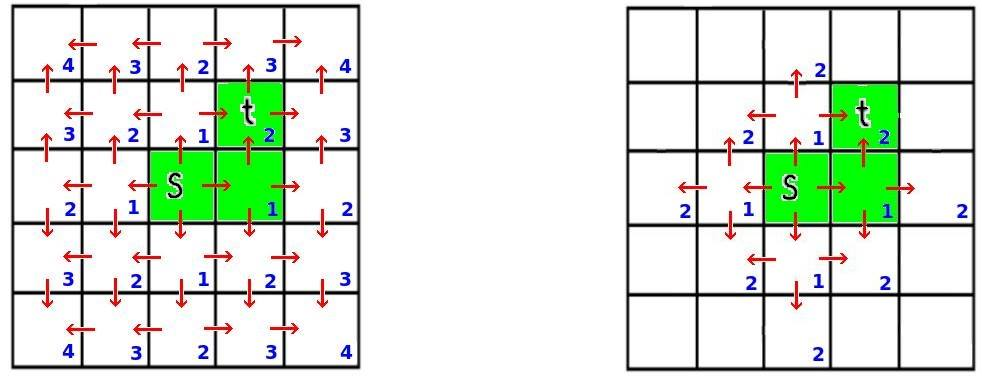
\includegraphics[scale=0.5]{dijkstra.png}
\caption{Dijkstra's algorithm vs. the modified Dijkstra's algorithm}
\end{figure}


%%%%%%%%%%%%%%%%%%%%%%%%%%%%%%% A* search %%%%%%%%%%%%%%%%%%%%%%%%%%%%%%%
\section{A* search}
A* search algorithm was developed in 1968 and is very similar to Dijkstra's algorithm. It examines an edge only once, and like Dijkstra's, A* will favor vertices who are close to the source vertex. The downside of Dijkstra's is however that the target vertex' direction is unknown. Thus, it might consider paths going in the complete opposite direction.\\
What makes A* better is that it uses heurestics to guide its search. Like the Greedy Best-first search algorithm, A* uses a heuristic function that can estimate how far away any vertex is from the goal. Vertices close to the goal are then favored over vertices who lie far away. However, Greedy Best-first search only uses the heuristic as information, when making a choice. By making a greedy decision based on only one criterion, the Best-first search algorithm runs considerably faster than Dijkstra's algorithm. The greedy solution is not always optimal though. By ignoring the distance moved so far, the algorithm may continue on a path it's on, even when the path has become very long.\\
A* is not greedy, since it keeps the estimated distance from source to vertex in mind, before extending the path. A* will therefore not be as fast as Greedy Best-First search, but will at least guarantee that a shortest path is found. By combining the information that Dijkstra's and Best-First search uses, A* search will be at least as fast as Dijkstra's algorithm, since the search can go in a more precise direction. This makes us able to minimize the number of vertices visited, before the target vertex is found. \\


%%%%%%%%%%%%%%%%%%%%%%%%%%%%%% Heuristics %%%%%%%%%%%%%%%%%%%%%%%%%%%%%%
\noindent\textbf{How A* search algorithm works}:\\
We wish to find the shortest path to a single target, so the pseudocode is based on the pseudocode for the modified Dijkstra's algorithm.\\

\textbf{A* Search$(G, w, s)$}
\begin{enumerate}
\NumTabs{24}
\setlength\itemsep{0em}
\item $d[s] = 0$
\item $S = Q = \{s\}$
\item $\textbf{while } Q \neq  $ \O
\item \tab{$u = $ EXTRACT-MIN$(Q)$}
\item \tab{\textbf{if } $u = t$}
\item \tab{}\tab{\textbf{Terminate}}
\item \tab{\textbf{for} each vertex $v \in G.Adj[u]$}
\item \tab{}\tab{\textbf{if } $v \notin S$}
\item \tab{}\tab{}\tab{INCREASE-KEY$(Q, v, d[v] + \|t-v\| ) $}
\item \tab{}\tab{}\tab{$S = S \cup \{v\}$}
\item \tab{}\tab{}\tab{$Q = Q \cup \{v\}$}
\item \tab{}\tab{}\tab{$d[v]  = d[u] + w(u,v)$}
\item \tab{}\tab{}\tab{$\pi[v] = u$}
\end{enumerate}
Explanation...To make sure that edges are relaxed properly, A* may only take non-negative edges...
The difference is now that we also use heurestics to guide our search. Recall that Dijkstra's algorithm selects which vertex to visit next, by extracting the vertex with the lowest shortest-path estimate. For A* search, we also want to examine the Euclidean distance from a vertex $v$ to the target vertex $t$ for all vertices, $\|t-v\|$. Thus, A* search will maintain a min-priority queue $Q$, where vertices are keyed by $d[v]+\|t-v\|$. By repeatedly selecting the vertex with the lowest sum, we can get a more precise path search. This is illustrated on the following figure: ...\\\\

\subsection{Heuristic function for A* search}
In short, A* search algorithm takes the following two functions in use:
$$g(n) = \text{exact cost of path from source vertex to any vertex } n$$
$$h(n) = \text{the heuristic estimated cost from any vertex } n \text{ to the goal}$$
Each time A* search chooses which vertex to pick, it extracts the vertex $n$ with the lowest $f(n) = g(n)+h(n)$. The heuristic function we use for A* is a function that takes a vertex $v \in V$  and the destination vertex t $\in$ V, computes and returns the euclidean distance from v to t.\\
The euclidean distance in an n-dimensional space on points v and t is computed thus:\\
$$\sqrt{\displaystyle\sum_{i=1}^{n} (v_i - t_i)^2}$$
As we primarily consider plannar graphs, the euclidean distance will be implmented using 2 dimensions thus:\\
$$\sqrt{(v_x - t_x)^2 + (v_y - t_y)^2}$$
\textbf{SLUT PÅ AFSNIT}\\


In the case where d[v] is relatively small with high eucledean distances, the A* search may choose to visit these, thus the worst-case of A* search is the modified dijkstra.\\\\



%%%%%%%%%%%%%%%%%%%%%%%%%%%% A* search proof %%%%%%%%%%%%%%%%%%%%%%%%%%%%
\newpage
\section{Correctness of A* search algorithm}\\
To prove that A* search algorithm work, we will perform an induction proof. Let $S$ be the set of vertices, whose shortest path have been found, $S=V-Q$.\\\\







\section{Running time analysis}
---

\section{Results}
\section{Bibliography}

\end{document}
